\documentclass[oneside]{book}
\usepackage{latexsym}

\usepackage{graphicx}
\usepackage{caption}
\usepackage{float}
\usepackage{amssymb}
\usepackage{amsfonts}
\usepackage{amstext}
\usepackage{amsthm}
\usepackage{amsmath}
\usepackage{tikz}
\usepackage{listings}
\usepackage{hyperref}
\usepackage{amsmath}
\usepackage{listings}
\usepackage{longtable}

\usepackage[margin=1.2in]{geometry}


\hypersetup{%
    pdfborder = {0 0 0}
}

\pagestyle{empty}
%\textwidth=13.5cm
%\textheight=21cm

\lstset{
  basicstyle=\fontsize{8}{10}\selectfont\ttfamily
}

\lstdefinestyle{customc}{
  belowcaptionskip=1\baselineskip,
  breaklines=true,
  xleftmargin=\parindent,
  language=C,
  showstringspaces=false,
  basicstyle=\footnotesize\ttfamily,
  keywordstyle=\bfseries\color{green!40!black},
  commentstyle=\itshape\color{purple!40!black},
  identifierstyle=\color{blue},
  stringstyle=\color{orange},
}

\lstdefinestyle{customg}{
  belowcaptionskip=1\baselineskip,
  breaklines=true,
  xleftmargin=\parindent,
  language={[x86masm]Assembler},
  showstringspaces=false,
  basicstyle=\footnotesize\ttfamily,
  keywordstyle=\bfseries\color{green!40!black},
  commentstyle=\itshape\color{purple!40!black},
  identifierstyle=\color{blue},
  stringstyle=\color{orange},
}


\frenchspacing
\begin{document}


%DEFINICJA SKLADANIA TWIERDZEN
\newtheorem{twr}{Twierdzenie}

\vspace{1cm}
\begin{center}
    \large
   	\textbf{Jakub Radlak}
\end{center}

\vspace{1.5cm}
\begin{center}
    \Large{\textbf{Orbital Flight Simulator \\ 
    - educational program \\
    Virtual Machine Description}}

\end{center}

\vspace{3.2cm}
\begin{center}
\large
Warsaw, April 2024
\end{center}

\newpage

% Wstawienie spisu treści:
\tableofcontents

\pagestyle{plain}

\chapter{On-board computer model - Virtual Machine}

The on-board computer is implemented as a sub-module of our simulation application. This is called a ``Virtual Machine'' with its own virtual memory, registers and instruction set. In addition, the VM has a byte-code interpreter and a translator from assembler to byte-code. This is all written in C++ and runs asynchronously in a separate thread. The application includes a simple assembly language code editor and offers the ability to load and save programs.

The figure \ref{fig:vm_schema} shows a general diagram of the Virtual Machine. In the following sections, we will discuss in detail the objects shown in this figure. That is: assembly code, translator, byte-code, interpreter, registers and main memory.

\begin{figure}[H]
    \centering
    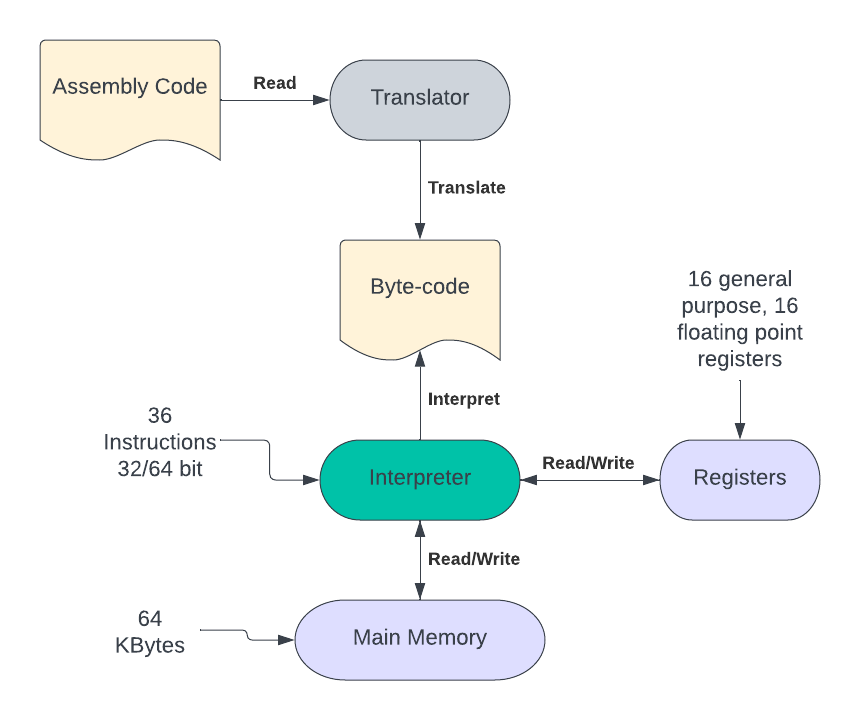
\includegraphics[width=0.7\textwidth]{Images/VMSchema2.png}
    \caption{Virtual Machine Schema, source: self-elaboration}
    \label{fig:vm_schema}
\end{figure}

\section{Main memory organisation}

The virtual machine contains 64 kilobytes of random access memory. Memory has no specific structure: it is represented as single-dimensional array of bytes. The interpretation of a series of bytes in memory depends on the context of the instruction. For example: it may be a floating point number, an integer number, a string, e.t.c. 
The memory class written in C++ contains several methods that enables to store and fetch data. Listing (5.1) shows methods for storing and retrieving double-precision floating-point numbers. Each number of this kind is 8 bytes in size.

%\begin{lstlisting}[language=c++, caption={Memory fetch and store}]
\begin{lstlisting}[caption=Fetch and store dword into memory, label={lst:mem-fetch}, language=C++, style=customc]
double Memory::fetchDWord(unsigned int addr) {
	assertConditions(addr + 8);
	unsigned char result[8] = { };
	memcopy(mem, result, addr, 0, 8);
	double val = *reinterpret_cast<double*>(result);
	leaseSemaphore();
	return val;
}

void Memory::storeDWord(unsigned int addr, double dword) {
	assertConditions(addr + 8);
	unsigned char* result 
	  = static_cast<unsigned char*>(static_cast<void*>(&dword));
	memcopy(result, mem, 0, addr, 8);
	leaseSemaphore();
}
\end{lstlisting}

\noindent 
The universal function \emph{memcopy} copies a series of bytes between the requested locations in memory. Both methods use the \emph{assertConditions} and \emph{leaseSematore} functions, which provide multi-threaded security in concurrent resource access situations.

The example in Listing \ref{lst:fld} shows a VM instruction that uses the \emph{fetchDWord} function to fetch a number from memory and store it in a floating point register. We will talk about the instructions in the later sections of this paper.

\begin{lstlisting}[caption=Method that load from the memory into the register, label={lst:fld}, language=C++, style=customc]
void Instructions::fld(unsigned char* args) {
	unsigned char r_src_addr = args[1];
	unsigned char r_dst_addr = args[0];
	unsigned int src_addr = registers[r_src_addr];
	double value = memory.fetchDWord(src_addr);
	registers.fl(r_dst_addr, value);
}
\end{lstlisting}

There are regions of memory that have special interpretation and treatment. The figure \ref{fig:vm_memory_map} shows the main memory organization.

\begin{figure}[H]
    \centering
    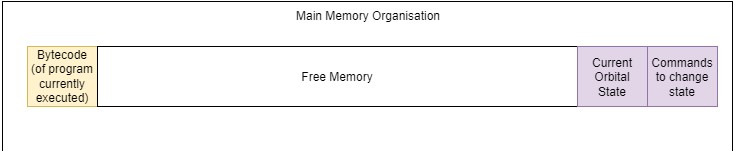
\includegraphics[width=1.0\textwidth]{Images/MemoryOrganisation.jpg}
    \caption{Map of the memory, source: self-elaboration}
    \label{fig:vm_memory_map}
\end{figure}

\noindent
The initial part of the memory is used to store the translated byte-code of the currently executing program. Usually it is from a few to several thousand bytes depending on the complexity of the program. Byte-code is represented as binary stream of bytes and it is very compact.
After byte-code there is the ``free space'' where programs can store their data, e.t.c.

Counting from the end, a few dozen bytes are used to store rocket flight telemetry information. This memory section is structured as follows:

\begin{lstlisting}
Rotation:
	z	65528
	y	65520
	x	65512
Velocity:	
	z	65504
	y	65496
	x	65488
Position:	
	z	65480
	y	65472
	x	65464
	
	mass	         65456
	thrust magnitude 65448
	altitude         65440
	timestamp        65432
\end{lstlisting}

\noindent 
The last few bytes are reserved to store temporary command data sent to the rocket.

\section{Registers organisation}

The virtual machine has 16 floating point registers and 16 general purpose registers. Floating point registers can store 64 bit double precision floating point numbers. The general purpose registers are 32 bits. So we can say that the VM has a hybrid 32/64 bit architecture and has a built-in FPU (Floating Point Unit).

In addition, there are three special-purpose registers:

\begin{itemize}

\item Zero Flag Register (ZF) - is used in compare and jump instructions. When the two compared values are equal, it takes the value 1.

\item Carry Flag Register (CF) - is used in comparisons and jump instructions. When the first of the compared values is greater than the second, the register is set to 1.

\item Program Counter (PC) - used to store the address of the currently executed instruction.

\end{itemize}

All arithmetic operations, comparisons and jumps are performed only on registers. Special VM instructions are needed to move data from memory to registers and vice versa.

\section{Instructions set}

We can divide instructions set into these seven categories:

\begin{itemize}

\item Data copy operations.

\item Saving and loading data to and from memory.

\item Arithmetic operations.

\item Logical operations.

\item Comparisons and conditional jumps.

\item Unconditional jumps.

\item Special instructions.

\end{itemize}

We will discuss each of those groups separately.
Table 5.1 lists each supported operations. Instructions with the letter ``h'' at the beginning operate on floating-point registers. the target register is always specified first.

\begin{longtable}{ |p{2.5cm}||p{3cm}|p{3cm}|p{2cm}| }
\caption{List of instructions}\\    %%%%<===
\hline
  Instruction name & Description & Arguments & Arguments size\\
 \hline
 \multicolumn{4}{|c|}{Data copy operations} \\
 \hline
  \hline 
	mov, fmov & Moves data between two registers & ids of destination and source registers & 2 x 8 bits\\
  \hline
	set, fset & Store value in the register & id of register, 32 or 64 bit value & 1 x 8 bits + 32 or 64 bits\\
  \hline  
  \multicolumn{4}{|c|}{Load and store data from and to memory} \\
 \hline
   \hline
 ld, fld, bld & Load value from the memory and store it into register & id of the destination register, id of the register in which address of value in memory is stored  &  2 x 8 bits \\
 \hline
 st, fst, bst & Store value from the register into memory & id of the register in which address of the destination in memory is stored, id of the register storing source value &  2 x 8 bits \\
 \hline
   \multicolumn{4}{|c|}{Arithmetical operations} \\
 \hline
   \hline
add, fadd, sub, fsub, mul, fmul, div, fdiv, mod & Add, subtract, multiply, divide and modulo two values and store result into the destination register  & ids of the source and destination registers &  2 x 8 bits \\
\hline
   \multicolumn{4}{|c|}{Logical operations} \\
 \hline
   \hline
vor, vand, vxor & Logical or, and, xor on two values and store result into the destination register  & ids of the source and destination registers &  2 x 8 bits \\
\hline
vnot & Logical not of single value & id of register which value must be negated & 1 x 8 bits \\ 
\hline
vshl, vshr & Shift bits in left or right direction & id of destination register, id of register in which number of bits to shift are stored& 2 x 8 bits \\ 
\hline
   \multicolumn{4}{|c|}{Comparisons and conditional jumps} \\
 \hline
   \hline
cmp, fcmp & Compare values of two registers. Sets ZF register to 1 if values are equal, and CF register if second register is greater than first & ids of registers to compare & 2 x 8 bits \\
\hline

 \hline
jz, jnz & Jump if ZF flag is set to 1 (jz) or is set to 0 (jnz) & id of register with address to jump & 1 x 8 bits \\
\hline

jc, jnc & Jump if CF flag is set to 1 (jv) or is set to 0 (jnv) & id of register with address to jump & 1 x 8 bits \\
\hline

jbe, ja & Jump if both ZF and CF flags are set to 1 (jbe) or CF is set to 1 and ZF is set to 0 (ja) & id of register with address to jump & 1 x 8 bits \\
\hline

\hline
   \multicolumn{4}{|c|}{Unconditional jumps} \\
 \hline

jmp & Unconditional jump & Address to jump & 32 bits \\
\hline

jmpr & Unconditional jump & id of register in which address to jump is stored & 1 x 8 bits \\
\hline

\hline
   \multicolumn{4}{|c|}{Special instructions} \\
 \hline
cmd & Send command to the rocket & id of register in which command code is stored, id of floating point register in which value of command is stored & 2 x 8 bits \\
\hline

halt & Stops Virtual Machine & & \\

\hline
ftc & Fetch the rocket's orientation and physical data, and store it to memory. & & \\
\hline

%\end{tabular}
\end{longtable}

\section{Assembly language}

The assembly language used by our on-board computer is a low-level language, similar in some respects to the Z80 or C64 assembly language described in \cite{z80} and \cite{mos}. Main difference is that our language supports floating point numbers and registers. The number of registers in our implementation is also much larger. The assembly syntax is very simple. Each non-blank row has the following structure:

\begin{lstlisting}
(db str)|label: |(instr (label|(idreg1 [(,)idReg2|value])))

where
   a | b  means alternative
    (a)   means requirement
    [a]   means optionality
   
   db     defines string of characters
   instr  is instruction name
   label  is any string of characters (excluding white spaces)
   value  is any number 
   idReg1 is first register identifier
   idReg1 is second register identifier   
\end{lstlisting}

As it turns out, a simple language and a set of instructions listed above is enough to code any algorithm. This means it is Turing-Complete. Comparison statements and conditional jumps are enough to implement branches and loops of any kind.

For example, the program in listing \ref{lst:hello} copies the string ``Hello world'' from program code memory to another address in VM memory.

\begin{lstlisting}[caption={Hello World assembly program}, label={lst:hello}, language=C++, style=customc]

; store address of data in register (Hello world literal)
set r4, data

; set up registers for memory addresses
vxor r0, r0
set r1, 1
set r3, 256

print_loop:
  ; fetch byte from addres stored in r4
  bld r2, r4

  ; if zero, exit the loop
  cmp r2, r0
jz .end

; otherwise store byte in desired address in memory
bst r3, r2
add r3, r1

; move r4 on another character and go back
; to the beginning of the loop
add r4, r1
jmp print_loop

.end:
  halt
data:
  db Hello world
\end{lstlisting}

\noindent
Lines starting with ``;'' are ignored and act as comments. Comments in Listing \ref{lst:hello} describe the function of each block of code.  
``db'' is not a instruction. This is a special directive for the translator, which means that the following string must be treated as a compact piece of memory and stored right after the translated program byte-code.

\section{Translator to byte-code}

Virtual Machine does not run assembly language code directly. Regardless of how cryptic the reading may seem, assembly language was designed to be used by a human, not a virtual machine interpreter. 
There are a two main reasons for this: 

\begin{itemize}

\item Assembly language written as text is still very verbose compared to other methods of storing computer programs in memory. This is all the more important since we only have 64 kilobytes of main memory.

\item The interpreter can become unnecessarily complicated if it has to translate and decode every single line of code individually. 

\end{itemize}

We need to translate our assembly code into something more convenient for execution by a relatively simple interpreter. Therefore, our virtual machine has a supporting subsystem that is able to generate a stream of binary data corresponding to our assembly source code. This binary data is called byte-code.

The bytecode has a relatively simple structure: each line is translated one-to-one into the following stream of bytes:

\begin{lstlisting}

opCode+argumentBytes

where
	opCode         is a numerical identifier 
	               of the instruction
	               
	argumentBytes  is a string of bytes representing
	               the arguments of the instruction
	               
	+              is an empty space - there is no
	               byte separation between 
	               nstrCode and argumentBytes
\end{lstlisting}

Each pair like above is stored next to other. It produces very compact stream: considering that each \emph{opCode} is exactly one byte, length of \emph{argumentBytes} is variable between 1 and 8 bytes. The interpreter knows the length of each \emph{opCode's} \emph{argumentBytes} because it uses a built-in table of instructions similar to the list we provided in the section above.

Listing \ref{lst:translate} shows an example translator method. It translates an instruction class that takes a register identifier and a floating point number as arguments. Such an instruction could be, for example, fset: (fset f9, -1.27)

\begin{lstlisting}[caption=Translate instruction, label={lst:translate}, language=C++, style=customc]
void Translator::trnsl_fconstant_to_register(
std::tuple<unsigned int, unsigned int> instr, std::string line) {
  // decode opcode and arguments size
  line = trim(line);
  unsigned int opcode = std::get<0>(instr);
  unsigned int instrSize = std::get<1>(instr) + 1;

  // decode register number:
  int pos = line.find(" ") + 2;
  int pose = line.find(",");
  std::string regNumber = line.substr(pos, pose - pos);
  unsigned char reg = stoi(regNumber);

  // decode floating point constant number:
  pos = line.find(",") + 2;
  pose = line.size();
  std::string constant = line.substr(pos, pose - pos);
  double cnst = 0;
  if (std::isdigit(constant[0]) || constant[0] == '-') {
    cnst = stod(constant);
  } else {
    // label pointing to address
    cnst = labelDict[constant];
  }

  // calculate current instruction addres, 
  // and copy opcode, registry and decoded number 
  // into memory
  unsigned int addr = instr_addr - instrSize;
  code[addr++] = opcode;
  code[addr++] = reg;

  unsigned char* word = static_cast<unsigned char*>
  (static_cast<void*>(&cnst));
    
  Memory::memcopy(word, code, 0, addr, 8);
}
\end{lstlisting}

The comments in the \ref{lst:translate} listing describe the functions of each section of code.
The sample method in \ref{lst:translate} is one of several types of decoding methods, all other types are listed below:

\begin{itemize}

\item trnsl\_constant\_to\_register similar to trnsl\_fconstant\_to\_register above but refers to integer numbers
\item trnsl\_register\_to\_register - translate instructions that operates on two registers
\item trnsl\_constant - translate instructions that operates only on constants or labels
\item trnsl\_register - translate instructions that operates only on one register
\item trnsl\_halt - translate halt instruction

\end{itemize}

\section{Byte-code interpreter}

The byte-code interpreter is a simple subsystem of the virtual machine, and on the other hand one of the most important. It contains the main execution loop. It sequentially fetches instructions one by one, decodes them, and executes them. The special register PC (Program Counter) indicates the memory address of the next instruction to be executed. PC is incremented on each iteration of the loop if there was no jump. Jump instructions can modify the PC register.

Thanks to the transfer of part of the work to the language translator, the interpreter may be simple and fast. Execution loop method is shown in the listing \ref{lst:execLoop}

\begin{lstlisting}[caption=Execution loop, label={lst:execLoop}, language=C++, style=customc]
void VMachine::executionLoop() {
  // fetching first opcode:
  threadFinished = 0;
  unsigned int opcode = memory->fetchByte(0);
  while (opcode != opcodes->getOpcode("halt") && !shouldStop) {
    while (pause); // wait

    // decode and execute instruction:
    unsigned int args_size = opcodes->getInstrSize(opcode);
    unsigned char* args = new unsigned char[args_size];
    Memory::memcopy(memory->mem, args, pc + 1, 0, args_size);
    instructions->call(opcode, args);
    delete[] args;

    pc = registers->pc();
    if (oldpc == pc) {
        // there was no jump - update program counter:
        pc += args_size + 1;
        registers->pc(pc);
    }
    oldpc = pc;

    // fetch another opcode
    opcode = memory->fetchByte(pc);
   }

   threadFinished = 1;
}

\end{lstlisting}

Comments in the code in \ref{lst:execLoop} describe the behaviour of the method. There is another interesting observation: conditional and unconditional jump instructions can change the program counter (PC) register. In this case, the execution loop method cannot increment PC - this is reflected in the ``if'' statement in the method.


\section{Examples of the Virtual Machine programs}

Two demo flight oasm programs are provided with the application.

\begin{itemize}
\item The first program is the control program for simple ballistic flight, the highest phase of which is above the atmosphere.

\item The second program controls orbital flight. The orbit is highly eccentric and unstable. In the flyby phase near the perigee of the orbit, the rocket enters the upper atmosphere, which causes the rocket to gradually decelerate. The apogee and perigee of the orbit decrease with each successive orbit - the rocket will eventually fall to the Earth.

\end{itemize}

Listing \ref{lst:ballistic} displays short ballistic program written in the Orbital Flight Simulator assembly language.

\begin{lstlisting}[caption=Ballistic program, label={lst:ballistic}, style=customg]
; wait one second before starting the engine:

fset f2, 1000
set r1, 65432
wait_1_second:
  ftc
  fld f1, r1
  fcmp f1, f2
jc wait_1_second

; set the engine thrust value and send the command to the rocket:

fset f3, 0.24
set r8, 1
cmd r8, f3

; wait for the rocket to reach an altitude of 1.5 km:

check_altitude_loop:
  ftc
  set r3, 65440
  fld f1, r3
  fset f2, 1.5
  fcmp f1, f2
jc check_altitude_loop

; set the register values needed to execute
; the trajectory change commands:

set r3, 3
set r1, 2
set r4, 20
set r5, 1
set r2, 0

; a loop responsible for sending a series of commands
; to the rocket about changing
; the direction of the thrust vector:

change_trajectory_Y:
  ftc
  fset f9, -1.27
  cmd r3, f9
  sub r4, r5
  cmp r4, r2
jnc change_trajectory_Y

; a series of instructions responsible for
; waiting 180 seconds:

set r1, 65432
fset f2, 180000
wait_180_seconds:
  ftc
  fld f1, r1
  fcmp f1, f2
jc wait_180_seconds

; after exceeding the time, sending a command
; to cut off the ignition
; (in practice, reducing it to the value of 0.001):

fset f3, 0.001
set r8, 1
cmd r8, f3

; the last loop waiting for the altitude to exceed 100 km,
; after exceeding it, the program stops:

set r3, 65440
fset f2, 100
finish_check_altitude:
  ftc
  fld f1, r3
  fcmp f1, f2
jc finish_check_altitude

halt
\end{lstlisting}

\noindent
Comments in the program code describe the actions of individual sections of the code. The idea of this program is to use short loops that send commands to change the rocket's trajectory or allow the program to wait for external conditions to occur. Trajectory changes occur at exact points in time or at exact points in altitude. The current altitude and time points are read from the main memory from specific addresses. These addresses are described in the memory organization section of this article.

The other two demo programs work in a similar way. However, there are more critical points in time and space to consider in their case. Rocket flight programming is often limited to checking the occurrence of certain conditions and, if they occur, performing appropriate calculations in order to decide on the commands transmitted to the rocket. The key elements to make a decision are: the real-time clock and telemetry data saved in real-time in the memory of the virtual machine.

\end{document}
